
\begin{frame}{مسئلهٔ چند وزیر}
\begin{itemize}\itemr
\item[-]
می‌خواهیم تعداد n وزیر را در یک صفحه شطرنج
\m{n \times n}
به گونه‌ای قرار دهیم که هیچ یک از وزیرها همدیگر را تهدید نکنند. به عبارت دیگر هیچ دو وزیری نباید در یک سطر یا ستون یا خط مورب مشترکی قرار بگیرند.
\item[-]
دنباله‌ای که در این مسئله به دنبال آن می‌گردیم، دنباله‌ای است از n مکان که n وزیر در آنها قرار گرفته‌اند. مجموعه‌ای که هر یک از عناصر دنباله می‌توانند از  اعضای آن مجموعه انتخاب شوند عبارت است از مجموعه‌ای شامل
\m{n^2}
مکان بر روی صفحهٔ شطرنج.
\item[-]
ویژگی معینی که این دنباله باید داشته باشد این است که هیچ دو مکان انتخاب شده‌ای بر روی یک خط افقی، عمودی یا مورب قرار نگیرد.
\item[-]
مسئلهٔ چند وزیر یا
n
وزیر،
 حالت کلی مسئلهٔ ۸ وزیر است که در آن ۸ وزیر در یک صفحه شطرنج استاندارد با تعداد
۸ $\times$ ۸
مکان قرار می‌گیرند.
\item[-]
در اینجا برای سهولت نمایش حالات مختلف مسئله ۴ وزیر را در نظر می‌گیریم.
\end{itemize}
\end{frame}


\begin{frame}{مسئلهٔ چند وزیر}
\begin{itemize}\itemr
\item[-]
روش پسگرد در واقع روشی است که در یک درخت
\fn{1}{tree}
به صورت عمق-اول
\fn{2}{depth-first}
جستجو می‌کند. پس ابتدا جستجوی عمق-اول در درخت را توضیح می‌دهیم.
\item[-]
فرض کنید درختی داریم که از تعدادی رأس و یال تشکیل شده است و می‌خواهیم همهٔ مسیرهای درخت را که با ریشه شروع می‌شوند و با یک برگ پایان می‌یابند بررسی کنیم.
\item[-]
در واقع دنباله‌هایی که در اینجا بررسی می‌کنیم دنباله‌هایی هستند که یک مسیر در درخت را نشان می‌دهند و با ریشه آغاز و با یکی از برگ‌ها پایان می‌یابند.
\end{itemize}
\end{frame}


\begin{frame}{مسئلهٔ چند وزیر}
\begin{itemize}\itemr
\item[-]
ابتدا به سراغ ریشهٔ درخت می‌رویم و ریشه را به عنوان اولین عنصر دنباله انتخاب می‌کنیم. سپس اولین فرزند از سمت چپ در سطح یک درخت را انتخاب می‌کنیم و اگر این رأس دارای فرزند بود اولین فرزند آن را در سطح دو انتخاب می‌کنیم. این کار را ادامه می‌دهیم تا به یک برگ برسیم. تا اینجا یک مسیر در درخت را بررسی کرده‌ایم. با فرض اینکه برگ در سطح n قرار دارد، به رأس پدر در سطح
\m{n-1}
باز می‌گردیم و فرزند دوم را انتخاب می‌کنیم. این کار را ادامه می‌دهیم تا مسیر دوم و به همین ترتیب همهٔ مسیرها در درخت را بررسی کنیم.
\end{itemize}
\end{frame}


\begin{frame}{مسئلهٔ چند وزیر}
\begin{itemize}\itemr
\item[-]
درخت زیر را در نظر بگیرید. با استفاده از روش پسگرد ابتدا مسیر
\m{(1,2,3)}
سپس
\m{(1,2,4,5)}
سپس
\m{(1,2,4,6)}
، و به همین ترتیب
\m{(1,2,7)}
،
\m{(1,8,9)}
،
\m{(1,8,10)}
، الی آخر بررسی می‌شوند.
\begin{figure}
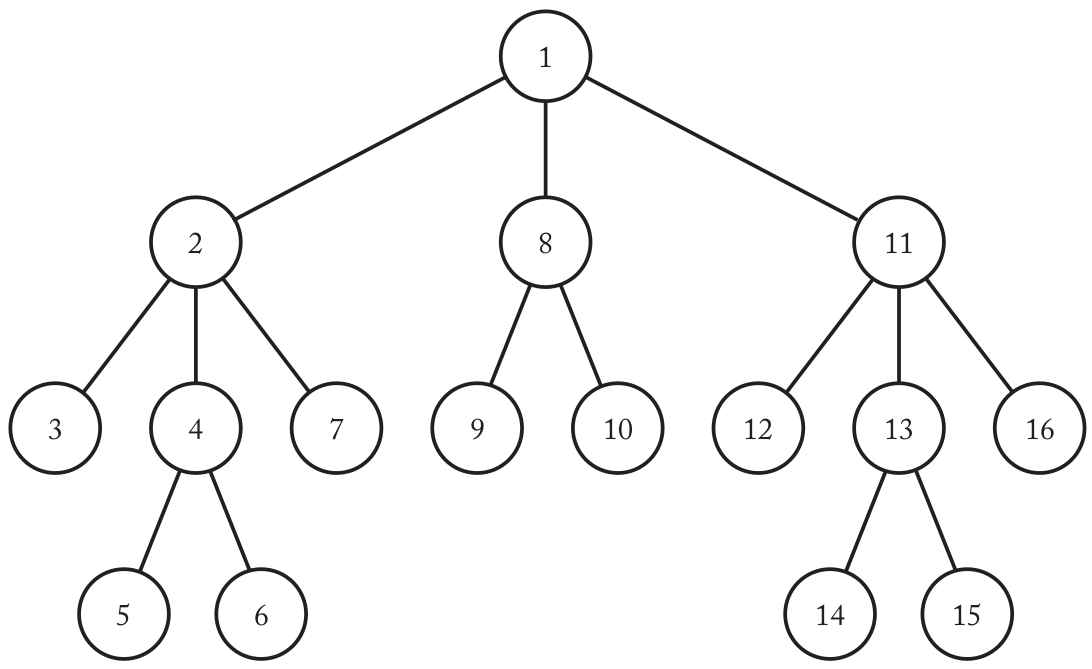
\includegraphics[width=0.6\textwidth]{figs/chap06/tree-backtrack}
\end{figure}
\end{itemize}
\end{frame}


\begin{frame}{مسئلهٔ چند وزیر}
\begin{itemize}\itemr
\item[-]
الگوریتم زیر این روش پسگرد را نشان می‌دهد.
\begin{algorithm}[H]\alglr
  \caption{Depth First TreeSearch} 
  \begin{algorithmic}[1]
   \Func{Depth-First-Tree-Search}{node v}
	 \State visit(v)
	 \For{each child u of v}
   			\State Depth-First-Tree-Search(u)
   	 \EndFor                     
  \end{algorithmic}
  \label{alg:merge}
\end{algorithm}
\end{itemize}
\end{frame}


\begin{frame}{مسئلهٔ چند وزیر}
\begin{itemize}\itemr
\item[-]
حال که با روش پسگرد آشنا شدیم، مسئلهٔ ۴ وزیر را در نظر می‌گیریم. می‌خواهیم ۴ وزیر را در یک صفحهٔ شطرنج
۴ $\times$ ۴
به گونه‌ای قرار دهیم که هیچ دو وزیری یکدیگر را تهدید نکنند. از آنجایی که هیچ دو وزیری نمی‌توانند در یک سطر قرار بگیرند، پس هر وزیر را باید در یک سطر متفاوت از بقیه وزیرها قرار دهیم. از آنجایی که هر وزیر در هر یک از ستون‌ها می تواند قرار بگیرد، بنابراین تعداد همهٔ حالت‌هایی که باید بررسی شوند برابر است با
۲۵۶ = ۴ $\times$ ۴ $\times$ ۴ $\times$ ۴.
\item[-]
برای بررسی همهٔ حالت‌ها درختی تشکیل می‌دهیم که در آن،
مکان اولین وزیر در سطح یک انتخاب می‌شود و مکان وزیر دوم در سطح دوم و به همین ترتیب مکان وزیر سوم در سطح سوم و مکان وزیر چهارم در سطح چهارم انتخاب می‌شوند.
\item[-]
یک مسیر از ریشه تا برگ درواقع یکی از گزینه‌های انتخاب مکان‌های صفحه را نشان می‌دهد. یک گزینه جواب مسئله است اگر در آن هیچ دو وزیری یکدیگر را تهدید نکنند.
\item[-]
به درخت تشکیل شده درخت فضای حالت گفته می‌شود.
\end{itemize}
\end{frame}


\begin{frame}{مسئلهٔ چند وزیر}
\begin{itemize}\itemr
\item[-]
قسمتی از درخت فضای حالات مسئله ۴ وزیر در شکل زیر نمایش داده شده است.
\begin{figure}
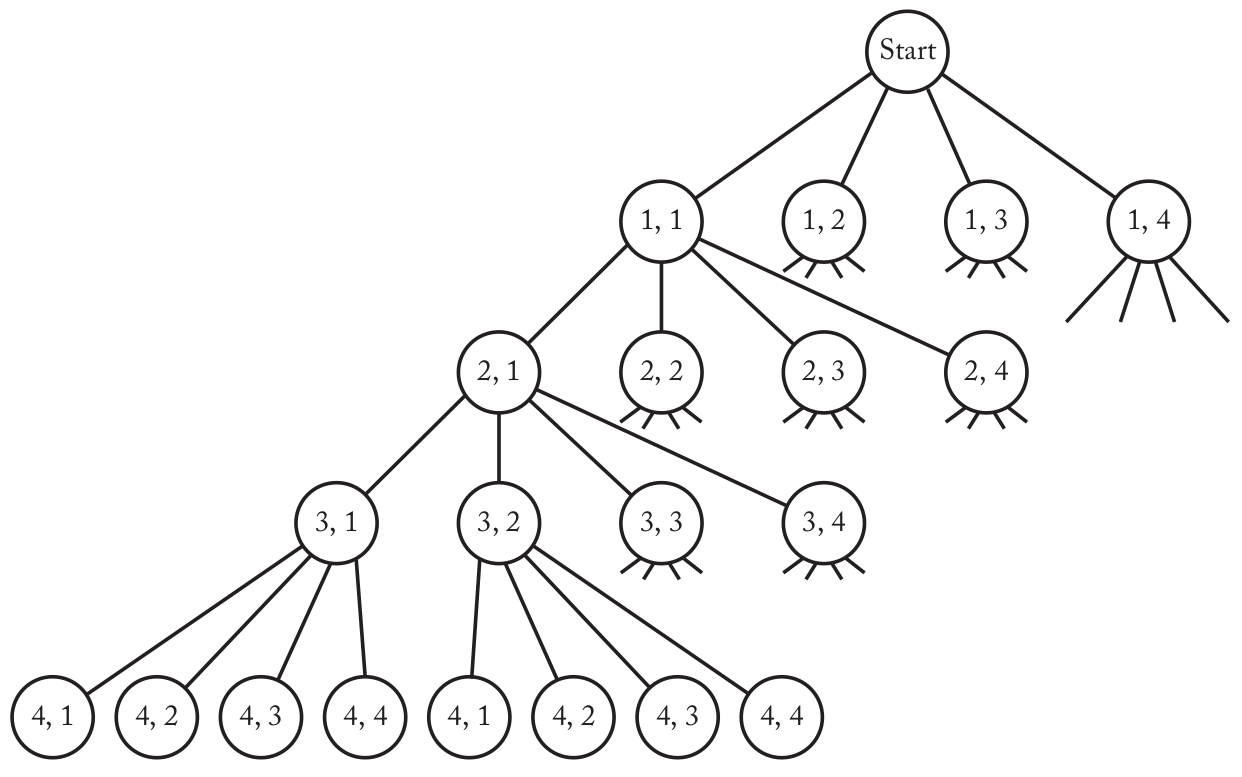
\includegraphics[width=0.7\textwidth]{figs/chap06/n-queens-tree}
\end{figure}
\end{itemize}
\end{frame}


\begin{frame}{مسئلهٔ چند وزیر}
\begin{itemize}\itemr
\item[-]
این درخت در مجموع ۲۵۶ برگ دارد که هر مسیر از ریشه تا یکی از برگ‌ها یکی از گزینه‌ها را نشان می‌دهد. در هریک از رأس‌های درخت یک جفت
\m{(i,j)}
ذخیره می‌شود که برابر با یک مکان در صفحهٔ شطرنج در سطر i و ستون j است.
\end{itemize}
\end{frame}


\begin{frame}{مسئلهٔ چند وزیر}
\begin{itemize}\itemr
\item[-]
 جستجو در این درخت می تواند بهینه‌تر از بررسی همهٔ ۲۵۶ انتخاب نیز انجام شود. برای مثال وقتی وزیر اول در مکان
\m{(1,1)}
قرار گرفت، بدیهی است که وزیر دوم نمی‌تواند در مکان
\m{(2,1)}
قرار بگیرد پس این مسیر در درخت ادامه داده نمی‌شود. همینطور وزیر دوم نمی‌تواند در مکان دوم قرار بگیرد پس نیازی نداریم این مسیر را نیز ادامه دهیم.
\item[-]
در شکل زیر این بهینه‌سازی نشان داده شده است.
\begin{figure}
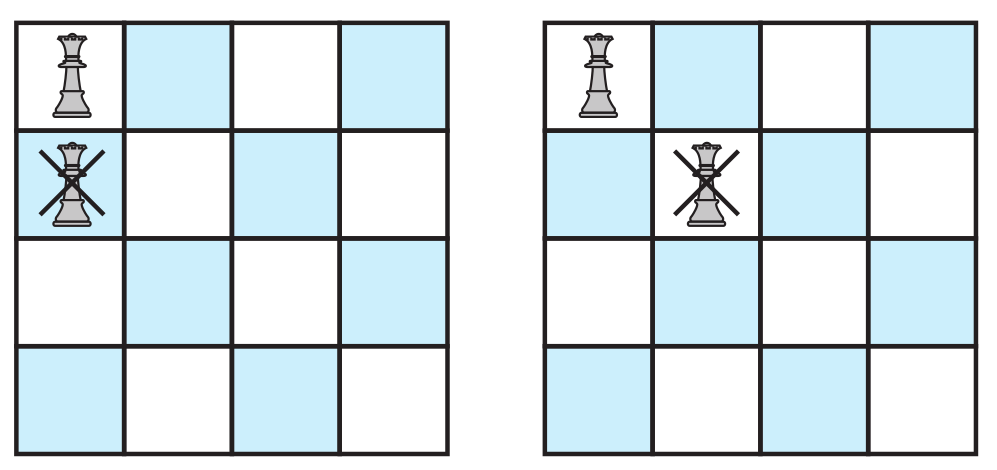
\includegraphics[width=0.6\textwidth]{figs/chap06/n-queens-opt}
\end{figure}
\end{itemize}
\end{frame}


\begin{frame}{مسئلهٔ چند وزیر}
\begin{itemize}\itemr
\item[-]
پسگرد عبارت است از روندی که توسط آن وقتی در یک انتخاب به یک گزینهٔ غیر جواب می‌رسیم، در درخت فضای حالت به عقب بازمی‌گردیم یا به عبارت دیگر از انتخاب یک رأس صرف نظر می‌کنیم و به رأس پدر پسگرد می‌کنیم تا فرزند بعدی پدر را انتخاب کنیم.
\item[-]
به یک رأس در درخت فضای حالت نومید کننده
\fn{1}{nonpromising}
می‌گوییم، اگر انتخاب آن رأس به جواب نیانجامد و به همین ترتیب به یک رأس امید دهنده
\fn{2}{promising}
می‌گوییم اگر با انتخاب آن همچنان احتمال رسیدن به جواب وجود داشته باشد.
\end{itemize}
\end{frame}


\begin{frame}{مسئلهٔ چند وزیر}
\begin{itemize}\itemr
\item[-]
به طور خلاصه در روش پسگرد، بر روی درخت فضای حالت، جستجوی عمق اول انجام می‌دهیم و در فرایند جستجو اگر به رأس نومید کننده برخورد کردیم مسیر را ادامه نمی‌دهیم و به رأس پدر پسگرد می‌کنیم.
\item[-]
به این روش هرس‌کردن
\fn{1}{pruning}
فضای حالت نیز گفته می‌شود که در آن تعدادی از دنباله‌ها بررسی نمی‌شوند.
\end{itemize}
\end{frame}


\begin{frame}{مسئلهٔ چند وزیر}
\begin{itemize}\itemr
\item[-]
در حالت کلی این الگوریتم به صورت زیر نوشته می‌شود.
\begin{algorithm}[H]\alglr
  \caption{Checknode} 
  \begin{algorithmic}[1]
   \Func{Checknode}{node v}
   \If{promising(v)}
   		\If{there is a solution at v}
   				\State write the solution
   		\Else
   			\For{each child u of v}
   					\State Checknode(u)
   			\EndFor
   		\EndIf
   	\EndIf                           
  \end{algorithmic}
  \label{alg:merge}
\end{algorithm}
\end{itemize}
\end{frame}


\begin{frame}{مسئلهٔ چند وزیر}
\begin{itemize}\itemr
\item[-]
ریشهٔ فضای حالت به تابع
Checknode
داده می‌شود که توسط آن رأس ریشه بررسی می‌شود. در بررسی یک رأس، ابتدا باید بررسی شود که انتخاب آن رأس امید دهنده است یا نومید کننده. اگر انتخاب آن امید دهنده بود و به جواب رسیدیم،‌ جواب را چاپ می‌کنیم. اگر انتخاب امید دهنده بود ولی به جواب نرسیدیم، رئوس فرزند به ترتیب برای بررسی انتخاب می‌شود.
\end{itemize}
\end{frame}


\begin{frame}{مسئلهٔ چند وزیر}
\begin{itemize}\itemr
\item[-]
تابع
promising
برای مسئله‌های مختلف متفاوت است. در مسئلهٔ ۴ وزیر، این تابع مقدار نادرست باز می‌گرداند اگر مکان‌های انتخاب شده از ریشه تا رأس مورد بررسی، به صورت سطری، ستونی یا قطری در یک راستا باشند.
\end{itemize}
\end{frame}


\begin{frame}{مسئلهٔ چند وزیر}
\begin{itemize}\itemr
\item[-]
در شکل زیر قسمتی از درخت فضای حالت به صورت هرس شده نشان‌داده شده است.
\begin{figure}
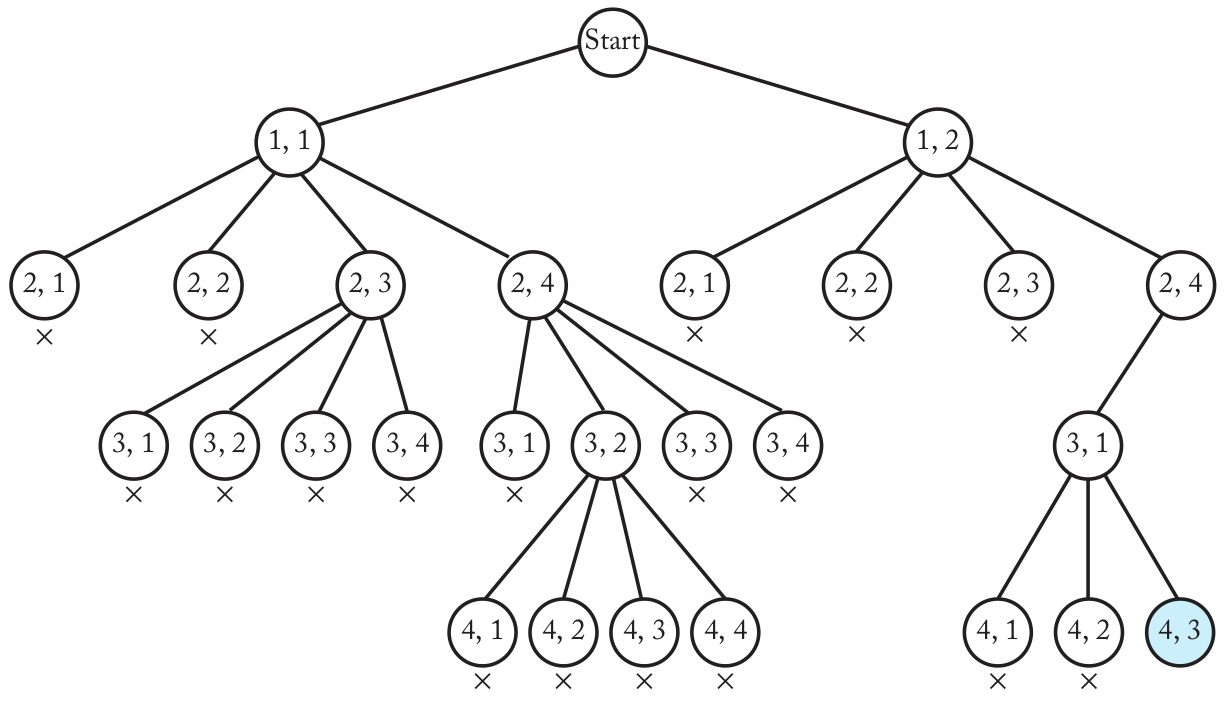
\includegraphics[width=0.7\textwidth]{figs/chap06/n-queens-tree2}
\end{figure}
\end{itemize}
\end{frame}


\begin{frame}{مسئلهٔ چند وزیر}
\begin{itemize}\itemr
\item[-]
در شکل زیر روند بررسی فضای حالت در صفحهٔ شطرنج نشان‌داده شده است.
\begin{figure}
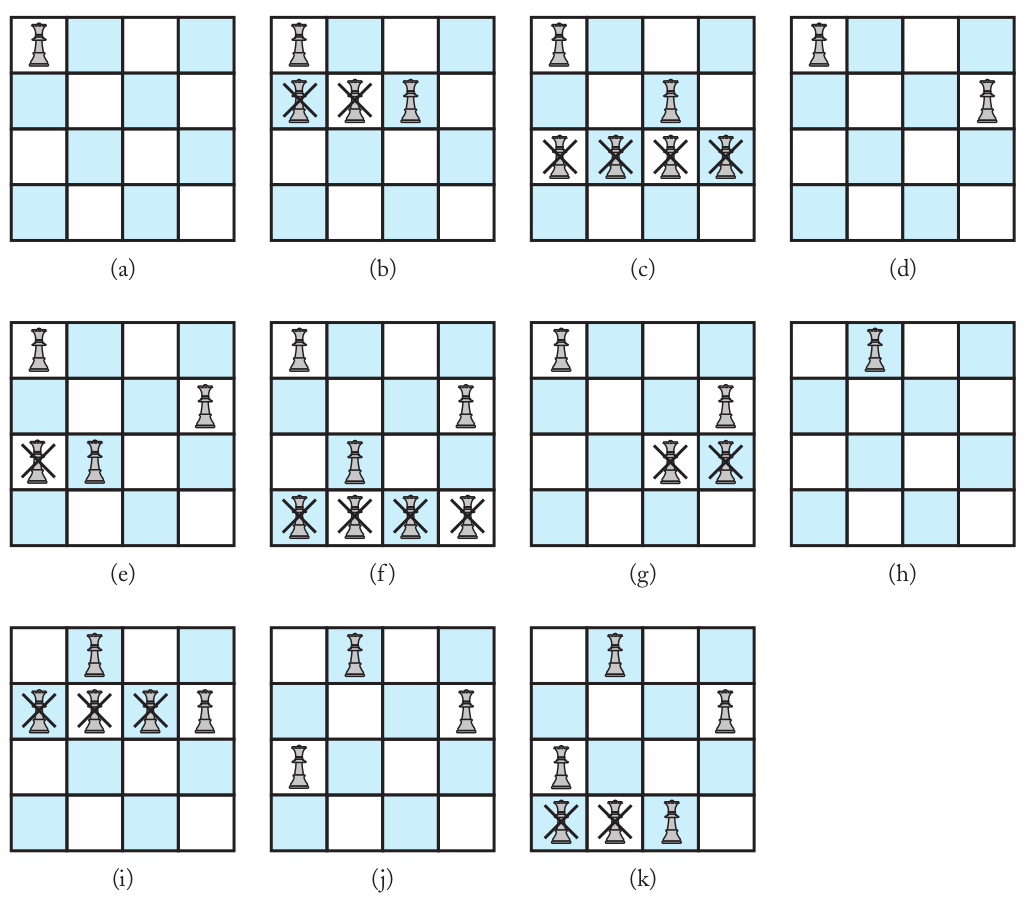
\includegraphics[width=0.5\textwidth]{figs/chap06/n-queens-board}
\end{figure}
\end{itemize}
\end{frame}


\begin{frame}{مسئلهٔ چند وزیر}
\begin{itemize}\itemr
\item[-]
تابع
promising
باید بررسی کند که آیا دو وزیر در یک ستون یا قطر قرار گرفته‌اند یا خیر.
\item[-]
اگر
\m{col(i)}
ستونی باشد که وزیر i ام در آن قرار گرفته است، باید بررسی کنیم که
\m{col(i)}
و
\m{col(j)}
برای هیچ دو وزیر i و j برابر نباشد.
\item[-]
همچنین دو وزیر به صورت مورب یکدیگر را تهدید می‌کنند اگر
\m{col(i) - col(j) = i - j}
و یا
\m{col(i) - col(j) = j - i}
باشد.
\end{itemize}
\end{frame}


\begin{frame}{مسئلهٔ چند وزیر}
\begin{itemize}\itemr
\item[-]
الگوریتم پسگرد برای مسئلهٔ چند وزیر به صورت زیر است. برای شروع الگوریتم تابع
\code{Queens(0)}
فراخوانی می‌شود.
\begin{algorithm}[H]\alglr
  \caption{Queens} 
  \begin{algorithmic}[1]
   \Func{Queens}{index i}
   \If{Promising(i)}
   		\If{i == n}
   				\State print col[1] through col[n]
   		\Else
   		\Statex \LeftComment{See if queen in (i+1)-st row can be}
   		\Statex \LeftComment{positioned in each of the n columns.}
   				\For{j = 1 \To n}
   					\State col[i + 1] = j
   					\State Queens(i + 1)	
   				\EndFor
   		\EndIf
  \EndIf                       
  \end{algorithmic}
  \label{alg:merge}
\end{algorithm}
\end{itemize}
\end{frame}


\begin{frame}{مسئلهٔ چند وزیر}
\begin{itemize}\itemr
\item[-]
\begin{algorithm}[H]\alglr
  \caption{Promising} 
  \begin{algorithmic}[1]
   \Func{Promising}{index i}
   \Statex  \LeftComment{Check if any queen k threatens queen in the i-th row.}	
   \For{k = 1 \To i - 1}	 
   			\If{col[i] == col[k] \textbf{or} |col[i] − col[k]| == i − k}
   					\State \Return false
   			\EndIf
   	\EndFor
   	\State \Return true                  
  \end{algorithmic}
  \label{alg:merge}
\end{algorithm}
\end{itemize}
\end{frame}


\begin{frame}{مسئلهٔ چند وزیر}
\begin{itemize}\itemr
\item[-]
حال می‌خواهیم الگوریتم پسگرد برای چند وزیر را تحلیل کنیم.
برای این کار تعداد رئوسی که در درخت فضای حالت بررسی می‌شوند را محاسبه می‌کنیم. از آنجایی که به دست آوردن تعداد دقیق حالات  وقتی حالت‌ها هرس می‌شوند ساده نیست، برای تعداد رئوس بررسی شده در درخت فضای حالت یک کران بالا در نظر می‌گیریم.
\item[-]
در درخت فضای حالات در سطح صفر، یک رأس داریم، در سطح یک تعداد n رأس، در سطح ۲ تعداد
\m{n^2}
رأس و در سطح n تعداد
\m{n^n}
رأس داریم. پس تعداد همهٔ رئوس بررسی شده برابر است با :
\begin{align*}
\m{1 + n + n^2 + n^3 + \cdots + n^n = \frac{n^{n+1} - 1}{n-1}}
\end{align*}
\item[-]
برای مسئله ۸ وزیر این تعداد برابر است با
\begin{align*}
\m{\frac{8^{8+1}-1}{8-1} = 19,173,961}
\end{align*}
\end{itemize}
\end{frame}


\begin{frame}{مسئلهٔ چند وزیر}
\begin{itemize}\itemr
\item[-]
حال یک کران بالای دیگر برای تعداد رئوس بررسی شده در نظر می‌گیریم. می‌دانیم که هیچ دو وزیری نمی‌توانند در یک ستون قرار بگیرند، بنابراین وقتی وزیر اول انتخاب شد، وزیر دوم تنها در ۷ مکان می‌تواند قرار بگیرد پس در سطح اول ۸ رأس و در سطح دوم
\LR{۸ $\times$ ۷}
رأس، در سطح سوم
\LR{۸ $\times$ ۷ $\times$ ۶}
رأس داریم و بدین ترتیب الی آخر.
\item[-]
پس در حالت کلی کران بالای رئوس بررسی شده برابراست با :
\begin{align*}
\m{1 + n + n(n-1) + n(n-1)(n-2) + \cdots + n!}
\end{align*}
\item[-]
برای مسئله ۸ وزیر این تعداد برابراست با
۱۰۹،۶۰۱
رأس.
\end{itemize}
\end{frame}


\begin{frame}{مسئلهٔ چند وزیر}
\begin{itemize}\itemr
\item[-]
تعداد دقیق رئوس بررسی شده را می‌توانیم با پیاده‌سازی الگوریتم به دست آوریم.
\item[-]
از آنجایی که کران بالای تعداد حالت مورد بررسی
\m{n!}
است، زمان اجرای الگوریتم پسگرد برای مسئلهٔ n وزیر
\m{O(n!)}
است.
\end{itemize}
\end{frame}